\documentclass[12pt]{article}
\usepackage{dsfont}
\usepackage{textcomp}
\usepackage{amsmath}
\usepackage{amssymb}
\usepackage{graphicx}
\usepackage{array}


\begin{document}


\title{Solutions to Sheet 10}
\author{Lukas Drexler, Leif Van Holland \\ \\
\textsc{Pattern Matching and Machine Learning} \\
\textsc{for Audio Signal Processing}}
\maketitle

\section*{Exercise 10.1}
\begin{center}
\begin{tabular}{c|c|c|c|c}
    $p$ & $F_{\text{pitch}}(p)$ & $F_{\text{pitch}}(p-0.5)$ & $F_{\text{pitch}}(p+0.5)$ & $BW(p)$ \\
    \hline
    60 & 261,63 & 254,18 & 269,29 & 7,67 \\
    61 & 277,18 & 269,29 & 285,30 & 8,12 \\
    62 & 293,66 & 285,30 & 302,27 & 8,61 \\
    63 & 311,13 & 302,27 & 320,24 & 9,12 \\
    64 & 329,63 & 320,24 & 339,29 & 9,66 \\
    65 & 349,23 & 339,29 & 359,46 & 10,23 \\
    66 & 369,99 & 359,46 & 380,84 & 10,84 \\
    67 & 392,00 & 380,84 & 403,48 & 11,49 \\
    68 & 415,30 & 403,48 & 427,47 & 12,17 \\
    69 & 440,00 & 427,47 & 452,89 & 12,89 \\
    70 & 466,16 & 452,89 & 479,82 & 13,66 \\
    71 & 493,88 & 479,82 & 508,36 & 14,47 \\
    72 & 523,25 & 508,36 & 538,58 & 15,33

\end{tabular}
\end{center}


\section*{Exercise 10.2}
For $p = 36$ we have $F_{\text{pitch}}(p-0.5) = 2^{\frac{35.5 - 69}{12}}\cdot 440 Hz \approx 63.544 \text{ Hz}$ and
$F_{\text{pitch}}(p+0.5) = 2^{\frac{36.5 - 69}{12}}\cdot 440 Hz \approx 67.323 \text{ Hz}$. We always have $F_{\text{coef}}(k) - F_{\text{coef}}(k-1) = F_{s} / N$. So if we want that $P(36)$ contains at least 4 coefficients, we need to ensure that \begin{align*}
&3 \cdot F_{s} / N &&\overset{!}{\leq} 67.323 - 63.544 = 3.779\\
\Leftrightarrow \qquad & F_{s} / N &&\overset{!}{\leq} 3.779 / 3 \approx 1.2596
\end{align*}
(Note that this condition is necessary but might not be sufficient. Requiring $4 \cdot F_{s} / N \leq 3.779$ is always sufficient, and in this case would lead to the same value of $N$)\\
So we need $N$ to be the smallest power that achieves this is $2^{15} = 32768$ (because $F_{s}/ 2^{14} \approx 1.346$).
Note that this also ensures that $P(48)$ contains at least 4 coefficients, as the intervals $\left[F_{\text{pitch}}(p-0.5),F_{\text{pitch}}(p+0.5)\right)$ only get larger for larger values of $p$.\\ 
So for $p=48$ we have $F_{\text{pitch}}(p-0.5) = 2^{\frac{47.5 - 69}{12}}\cdot 440 Hz \approx 127.089 \text{ Hz}$ and
$F_{\text{pitch}}(p+0.5) = 2^{\frac{48.5 - 69}{12}}\cdot 440 Hz \approx 134.646 \text{ Hz.}$\\
Therefore, $P(48) = \lbrace 189,190,...,199,200 \rbrace$, because $F_{\text{coef}}(188) \approx 126.51 < 127.089$, $F_{\text{coef}}(189) \approx 127.18 \geq 127.089$, $F_{\text{coef}}(200) \approx 134.58 < 134.646$, and $F_{\text{coef}}(201) \approx 135.26 \geq 134.646$. Clearly, for all values of $p$ between $189$ and $200$, $F_{\text{coef}}(p)$ has to lie in the interval.



\section*{Exercise 10.3}
\subsection*{b)}
    \begin{center}
        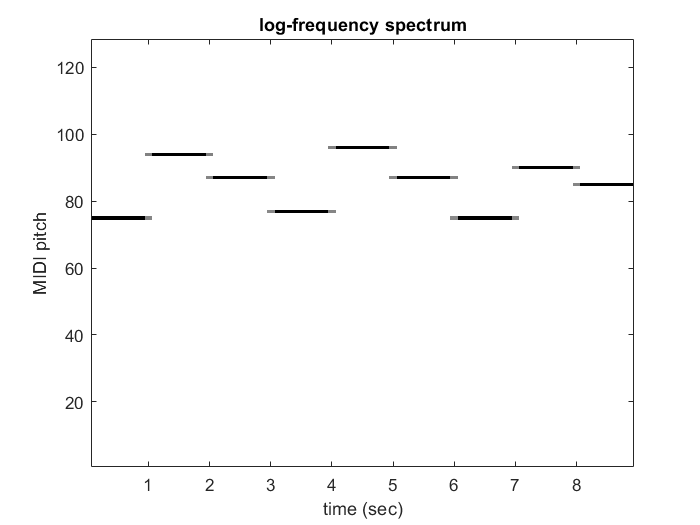
\includegraphics[width=\linewidth]{logspectrum}
    \end{center}

\subsection*{c)}
\begin{center}
    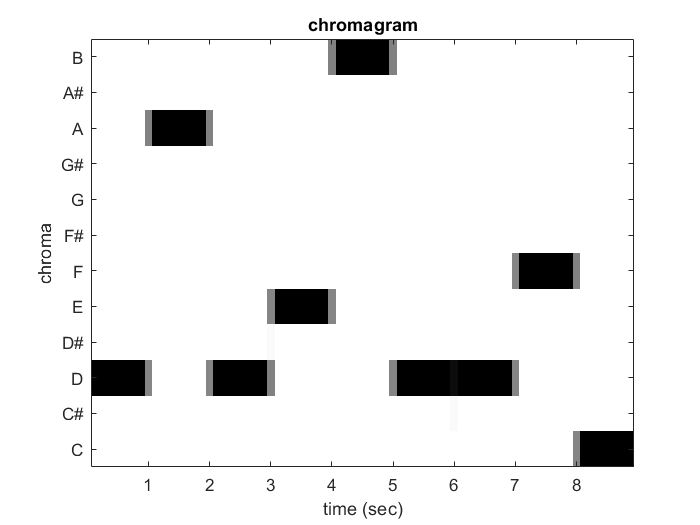
\includegraphics[width=\linewidth]{chromagram}
\end{center}

\end{document}
